\section{Исследования фазовых переходов и термодинамических свойств часовой модели с числом состояний спина \texorpdfstring{$q = 5$}{q=5}}

% \begin{abstract}
%    С помощью алгоритма Ванга-Ландау метода Монте-Карло проведены исследования фазовых переходов и термодинамических свойств часовой модели с числом состояний спина $q = 5$ на треугольной решетке. Используя гистограммный метод проведен анализ фазовых переходов. Показано, что в ферромагнитной часовой модели наблюдаются два фазовых перехода типа Березинского-Костерлица-Таулеса, а в антиферромагнитной часовой модели обнаружен фазовый переход второго рода.
% \end{abstract}

%\section*{Введение}
%
%Исследование фазовых переходов (ФП), магнитных, термодинамических и критических свойств в магнитных спиновых системах представляет большой теоретический и экспериментальный интерес. Это связано с тем, что для большинства реальных магнитных спиновых систем характерны возмущения различной природы, такие как анизотропия, взаимодействия следующих за ближайшими соседей, внешнее магнитное поле, тепловые и квантовые флуктуации, немагнитные примеси, дефекты, деформации и др. Присутствие этих факторов может повлиять на природу ФП и термодинамические характеристики таких систем \cite{bib:rmk-1, bib:rmk-2, bib:rmk-3}. Для изучения особенностей термодинамического поведения и природы ФП успешно используются различные решеточные модели. На их основе получено большое количество интересных результатов. Решеточные спиновые модели позволяют описать целый ряд реальных магнитных материалов.
%
%Одной из моделей, применяемых для описания физических систем, является часовая модель с числом состояний спина $q$. Нами в данном исследовании рассматривается часовая модель с числом состояний спина $q=5$ на треугольной решетке. Магнитные материалы на треугольной решетке представляют особый интерес для исследователей. Антиферромагнетики на треугольной решетке представляют собой геометрически фрустрированные спиновые системы, которые исследуются уже давно. Для фрустрированных систем существует совсем немного надежно установленных фактов. Большинство имеющихся результатов получены для модели Изинга, Гейзенберга и Поттса с числом состояний спина $q = 2$, $3$ и $4$ \cite{bib:rmk-4, bib:rmk-5, bib:rmk-6}.
%
%Многие физические свойства часовой модели зависят от значения $q$. В случае, когда $q = 2$, $3$, $4$, эта модель имеет точное решение. Установлено, что для этих трех случаев в системе наблюдается ФП второго рода из высокотемпературной парамагнитной фазы в низкотемпературную ферромагнитную упорядоченную фазу. Когда $q \to \infty$ данная модель сводится к стандартной $XY$ модели. В этом случае спонтанного нарушения симметрии не наблюдается, но происходит ФП из низкотемпературной фазы Березинского-Костерлица-Таулеса (БКТ) в высокотемпературную парамагнитную фазу. Для часовой модели с числом состояний спина $q = 5$ имеется очень мало точно установленных фактов. К настоящему моменту остается открытым вопрос о роде ФП при значении $q = 5$.
%
%Для получения ответа на этот вопрос в данной работе нами проводится исследование двумерной часовой модели на треугольной решетке с $q = 5$. Исследование этой модели с антиферромагнитными обменными взаимодействиями на треугольной решетке в литературе практически не встречается. Антиферромагнитное обменного взаимодействие в данной модели может привести к фрустрации, вырождению основного состояния, появлению различных фаз и ФП, а также влиять на его термодинамические, магнитные и критические свойства. В связи с этим в данной работе нами предпринята попытка провести исследование ФП и термодинамических свойств этой модели на треугольной решетке.
%
%Исследования проводятся на основе современных методов и идей, что позволит получить ответ на ряд вопросов, связанных с природой ФП и термодинамическим поведением фрустрированных спиновых систем.
%
%\section*{Результат исследования}

На рис.~\ref{fig:rmk-1} приведены температурные зависимости энтропии $S$.

\begin{figure}[ht]
    \begin{subfigure}{0.5\textwidth}
        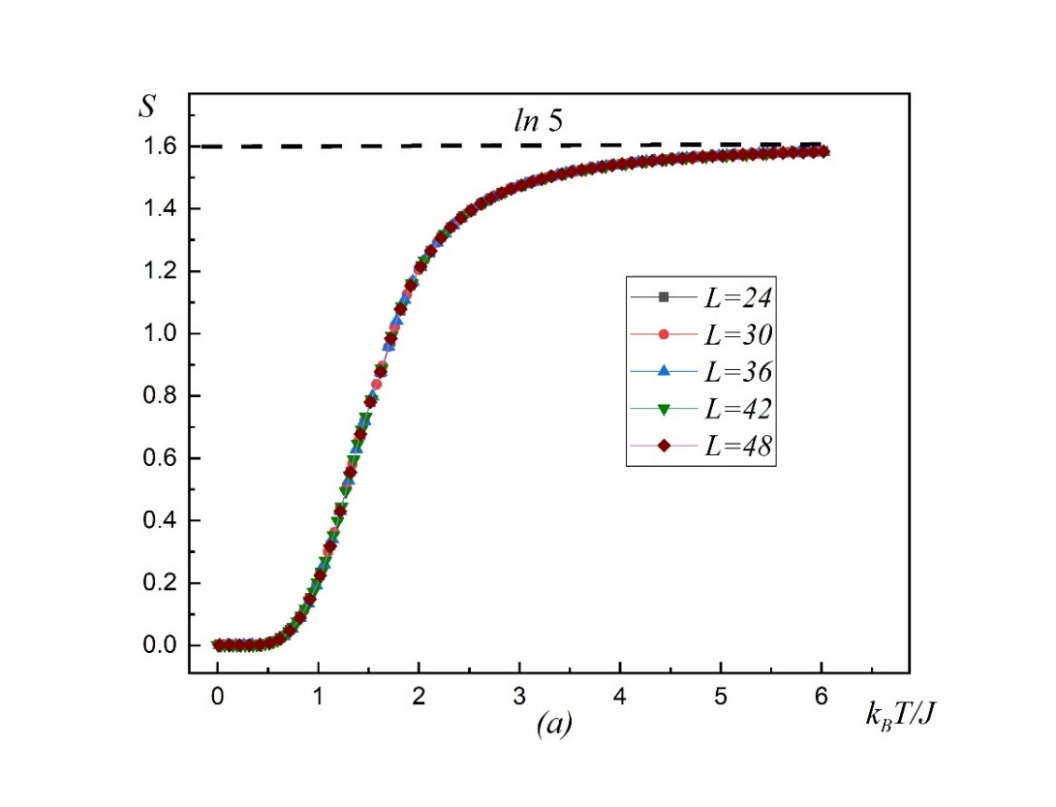
\includegraphics[width=\linewidth]{rmk/image1.jpeg}
        \caption{}
    \end{subfigure}
    \begin{subfigure}{0.5\textwidth}
        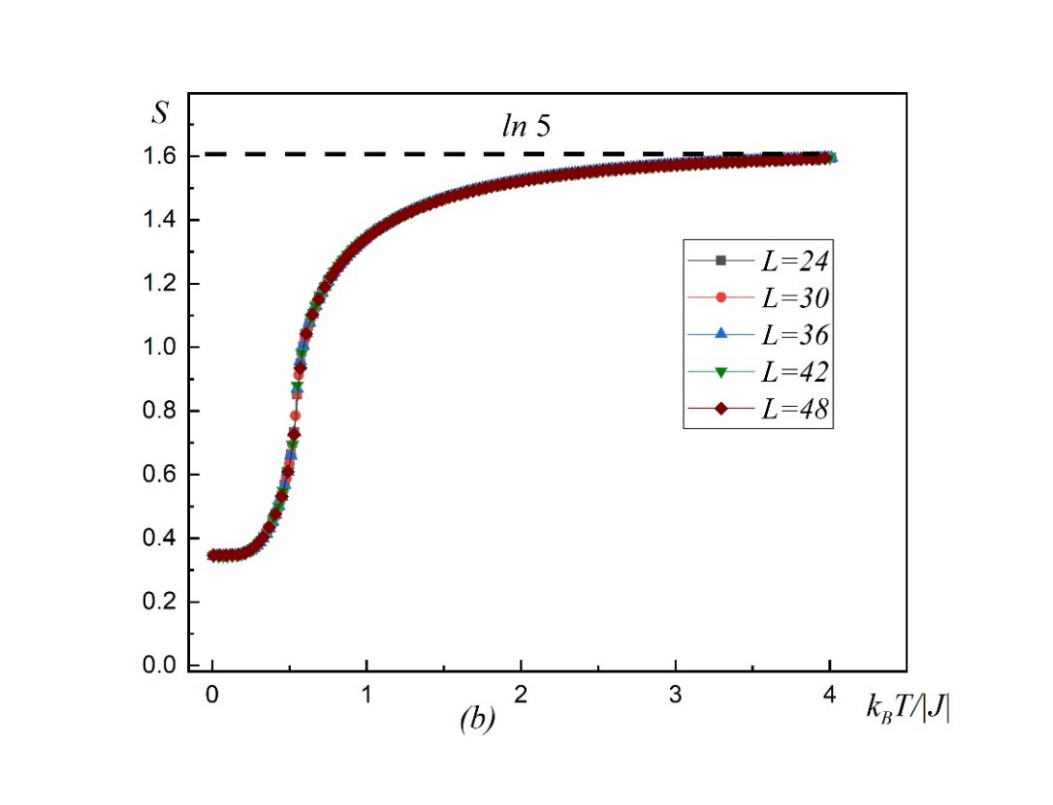
\includegraphics[width=\linewidth]{rmk/image2.jpeg}
        \caption{}
    \end{subfigure}
    \caption{Температурные зависимости энтропии S. a) для ферромагнитной модели; b) для антиферромагнитной модели.}
    \label{fig:rmk-1}
\end{figure}

Из рисунков видно, что с увеличением температуры энтропия для всех систем стремится к теоретически предсказанному значению $\ln 5$. При низких температурах, близких к абсолютному нулю, для ферромагнитной модели энтропия стремится к нулевому значению для всех значений $L$. Нулевая остаточная энтропия свидетельствует об отсутствии вырождения основного состояния. Для антиферромагнитной модели энтропия при низких температурах стремится к ненулевому значению для всех значений $L$. Такое поведение свидетельствует о сильном вырождении данной модели, что характерно для фрустрированных систем.

\begin{figure}[ht]
    \begin{subfigure}{0.5\textwidth}
        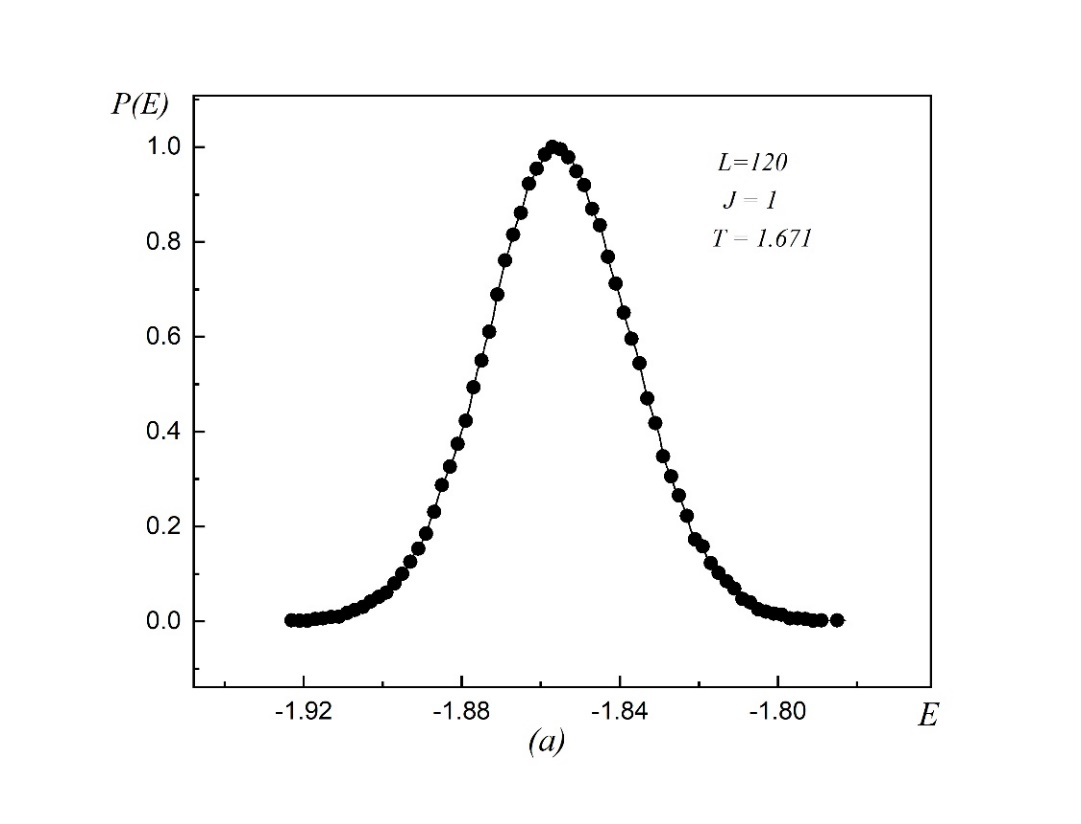
\includegraphics[width=\linewidth]{rmk/image3.jpeg}
        \caption{}
        \label{fig:rmk-2:a}
    \end{subfigure}
    \begin{subfigure}{0.5\textwidth}
        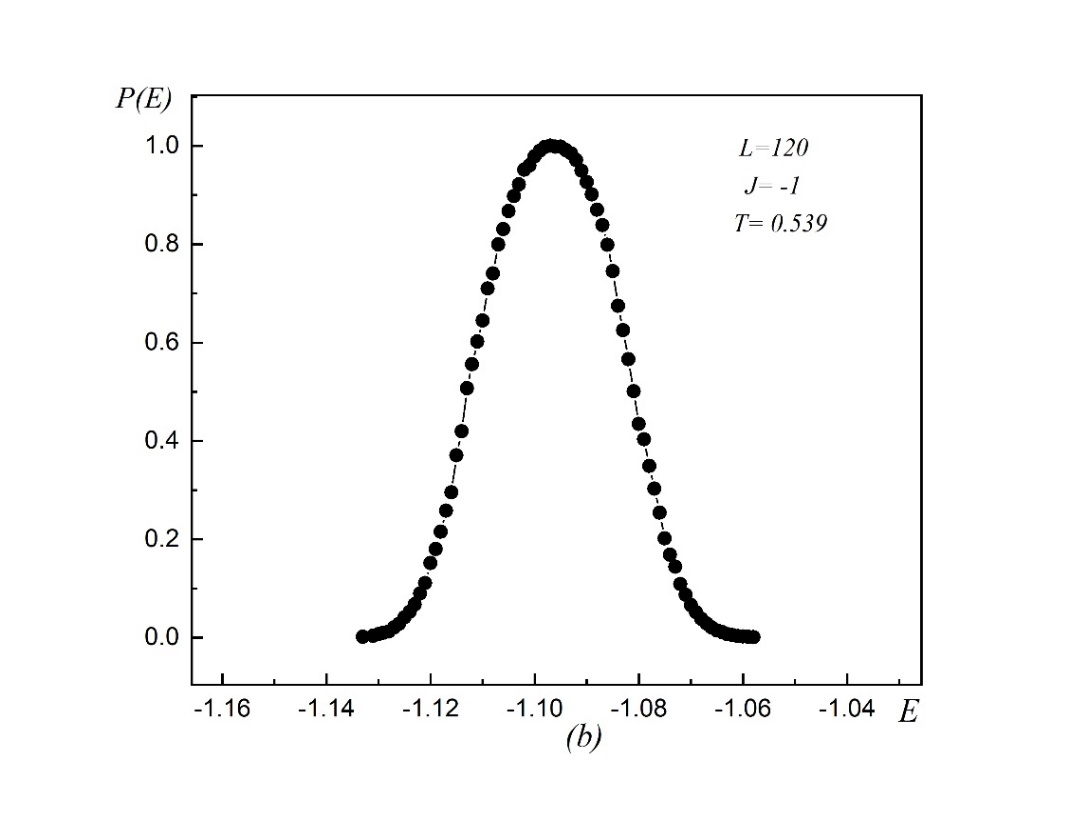
\includegraphics[width=\linewidth]{rmk/image4.jpeg}
        \caption{}
        \label{fig:rmk-2:b}
    \end{subfigure}
    \caption{Гистограмма распределения энергии. a) для ферромагнитной модели; b) для антиферромагнитной модели.}
    \label{fig:rmk-2}
\end{figure}

Для определения рода ФП мы использовали гистограммный анализ данных метода Монте-Карло. В случае ФП первого рода на гистограмме распределения энергии вблизи температуры перехода наблюдается бимодальное распределение энергии. То есть, на графике появляются два максимума, расположенных симметрично относительно равновесного значения энергии. В случае ФП второго рода должен наблюдаться один максимум. На рис.~\ref{fig:rmk-2:a} и \ref{fig:rmk-2:b} представлены гистограммы распределения энергии для линейных размеров системы $L=120$ в области температуры ФП для ферромагнитной и антиферромагнитной моделей. На графиках зависимости вероятности $P$ от энергии системы $E$ наблюдается один хорошо выраженный максимум, который свидетельствует о наличии в антиферромагнитной модели ФП второго рода. Для ферромагнитной часовой модели подобный анализ показывает наличие одного максимума, который позволяет нам утверждать, что в данной модели точно не наблюдается ФП первого рода. Такое поведение характерно для ФП второго рода.

%\section*{Заключение}
%
%Проведено исследование фазовых переходов и термодинамических свойств двумерной часовой модели на треугольной решетке с числом состояний спина $q = 5$ с использованием алгоритма Ванга-Ландау метода Монте-Карло. На основе гистограммного метода проведен анализ рода ФП данной модели. Обнаружено, что для ферромагнитной часовой модели происходят два фазовых перехода типа Березинского-Костерлица-Таулеса. Данные полученные для антиферромагнитной часовой модели свидетельствуют о том, что основное состояние системы сильно вырождено и в системе происходит ФП второго рода. Показано, что антиферромагнитное обменное взаимодействие ближайших соседей может повлиять на физические свойства часовой модели с $q=5$.
